\documentclass[12pt,a4paper]{report}
\usepackage[brazil]{babel}
\usepackage[]{algorithm}
\usepackage[]{algorithmic}

\usepackage[style=numeric,backend=biber]{biblatex}
\usepackage[utf8]{inputenc}
\usepackage{kpfonts}
\usepackage[T1]{fontenc}
\usepackage{wrapfig}
\usepackage{graphicx}
\usepackage{enumerate}
\usepackage{subcaption}
\usepackage{float}
\usepackage{caption}
\usepackage{listings}
\usepackage{lipsum}
\usepackage{amsthm}
\usepackage{amssymb}
\usepackage{bm}
\usepackage{color}
\usepackage{afterpage}
\usepackage[inline]{enumitem}
\usepackage{pdflscape}
\usepackage{listingsutf8}
\usepackage{siunitx}
\usepackage{bashful}

\usepackage{hyperref}
\hypersetup{
    colorlinks=true,
    linkcolor=blue,
    filecolor=magenta,      
    urlcolor=cyan,
}

\usepackage[margin=1in]{geometry}

\lstset{frame=tb,
  aboveskip=2mm,
  belowskip=2mm,
  showstringspaces=false,
  columns=flexible,
  basicstyle=\footnotesize,,
  numbers=left,
  numbersep=5pt,
  stepnumber=1,
  breaklines=true,
  keepspaces=true,
  breakatwhitespace=true,
  showtabs=false,  
  tabsize=2
}


% Definindo estilo para os códigos
\definecolor{mGreen}{rgb}{0,0.6,0}
\definecolor{mGray}{rgb}{0.5,0.5,0.5}
\definecolor{mPurple}{rgb}{0.58,0,0.82}
\definecolor{dkgreen}{rgb}{0,0.6,0}
\definecolor{backgroundColour}{rgb}{0.97,0.97,0.97}

\lstset{basicstyle=\ttfamily,
    backgroundcolor=\color{backgroundColour},   
    commentstyle=\color{mGreen},
    keywordstyle=\color{magenta},
    numberstyle=\tiny\color{mGray},
    commentstyle=\color{dkgreen},
    stringstyle=\color{mPurple},
    basicstyle=\footnotesize,
    breakatwhitespace=false\textbf{,}         
    breaklines=true,                 
    captionpos=b,                    
    keepspaces=true,                 
    numbers=left,                    
    numbersep=5pt,                  
    showspaces=false,                
    showstringspaces=false,
    showtabs=false,                  
    tabsize=2,
    language=bash
}

\lstdefinestyle{BStyle}{
    backgroundcolor=\color{backgroundColour},  
    showstringspaces=false,
    numbers=none,
    language=bash
}

\pagenumbering{arabic}
\renewcommand{\thesection}{\arabic{section}}

\bibliography{ref}
\renewcommand{\contentsname}{Sumário}{\thispagestyle{empty}}
\renewcommand{\baselinestretch}{1.5} 

\begin{document}

\begin{titlepage}
        \begin{center}
                \vspace*{1cm}
                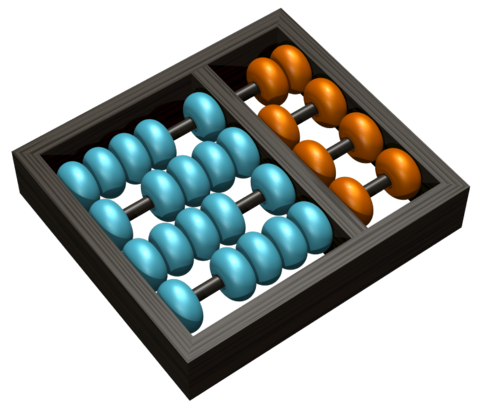
\includegraphics[width=0.25\textwidth]{Logo}\\
                \vspace{1.5cm}
                \Huge
                \textbf{Exercício 5}\\
                \vspace{1.5cm}
                \Large
                \textbf{Aluno}: João Vitor Gonçalves\\
                \textbf{RA}: 176353\\
                \vspace{1.2cm}
                \Large
                Instituto de Computação\\
                Universidade Estadual de Campinas\\
                \vspace{1.5cm}
                Campinas, 19 de Dezembro de 2020.
        \end{center}
\end{titlepage}
\tableofcontents
\clearpage

\newcommand{\shellcmd}[1]{\texttt{\footnotesize\# #1}}%estilizando citação de comandos do shell

\section{Cite um exemplo para uso de multiplexação de entrada e saída.}
Como sabemos, podemos usar a multiplexação de entrada e saída para podermos realizar operações de entrada e saída de forma não bloqueante.

Então por exemplo, podemos monitorar multiplas entradas de dados paralelamente sem bloquear o processo, como ler ao mesmo tempo de um arquivo e da entrada padrão, sem necessidade de criar processos filhos ou threads separadas, assim economizando recursos.

Algumas ferramentas de desenvolvimento web, como o NodeJS utilizam como padrão a multiplexação de entrada e saída para atender requisições de múltiplos clientes num servidor, tendo apenas um processo e thread principais.

\section{Compilação e execução}

Para realizar a compilação da aplicação, basta executar o script \emph{build.sh} fornecido.

\begin{lstlisting}[language=bash]
    ./lab/build.sh
\end{lstlisting}

Será criada uma pasta \emph{build} com os binários dos processos.

Para executar o servidor basta executar:

\begin{lstlisting}[language=bash]
    ./lab/build/server/server [PORT]
\end{lstlisting}

Para executar o cliente basta executar:
\begin{lstlisting}[language=bash]
    ./lab/build/client/client [IP] [PORT] < IN_FILE > OUT_FILE
\end{lstlisting}

O cliente irá enviar o conteúdo do arquivo para o servidor e receber os dados do mesmo paralelamente por meio de multiplexação de entrada e saída. Quando essa transferência for finalizada, o processo irá terminar.

O servidor suporta multiplos clientes conectados por meio de multiplexação de entrada e saída, com no máximo 100 clientes conectados simultaneamente.

\end{document}